\chapter{User Study: Design and Results}

\begin{quote}
\textbf{Status note.} This study pre-registered a target of 20 analysed participants, run to a
frozen protocol after a formal pass/fail pilot. \textit{Pre-registered} is used throughout in the
sense defined in Chapter 1, Section 1.4. Collection ended at \textbf{eighteen people tested},
across an initial pilot day and six further collection days, when the dissertation deadline arrived,
preceded by informal naive-pilot iteration used to tune stimulus parameters ahead of the frozen
protocol. Stopping two short of target is a protocol deviation and is reported as one. The analysis
proceeds because the achieved sample already delivers the sensitivity the design planned for: the
primary contrast and the pre-registered eccentricity band both reach the 80\% power level the
20-participant target was chosen to provide. Seventeen usable pairs exist for the workstation block
and fifteen for the driving block. Section 5.7 reports the final analysis of those pairs, read
against the pre-committed decision table, with the sample-size deviation carried into every verdict
rather than repeated sentence by sentence.
\end{quote}

\section{What the Study Must Be Able to Conclude}

The purpose of this study is to determine whether the system of Chapters 3 and 4 \textit{works},
and just as importantly to be able to determine that it \textit{does not}. A study that could only
confirm would be a demonstration rather than an experiment. Two design choices commonly produce that
defect: an underpowered between-subjects comparison, and safety hypotheses phrased as bare nulls,
since a non-significant difference in a small sample carries little evidential weight.

The design maps every outcome to a pre-committed conclusion by reframing the question around an
effect already established in the literature. Peripheral visual distractors reliably impose a
measurable performance cost on a focal sustained-attention task in a head-mounted display: in a
virtual-classroom Go/No-go study, commission errors more than doubled in the presence of peripheral
distractor events \citep[N = 66]{ai2025}. The primary question is therefore not the unconstrained
``does the vignette make people better?'' but the falsifiable:

\begin{quote}
\textit{Peripheral distractors impose a measurable cost on a focal task. Does the DR vignette reduce
that cost?}
\end{quote}

Under this framing every outcome is informative. The design relies on that established literature for
confidence that the distractor reel imposes a real cost, rather than on an internal manipulation
check, and that dependency is carried into the limitations.

Two methodological commitments govern the study's position. The driving block is a
\textbf{simulation}, with participants viewing pre-recorded equirectangular footage rather than a
live street, in the tradition established by \citet{cheng2022}, which gives every participant
identical, repeatable, event-dense stimuli at a declared cost to ecological validity. And detection
comes from the \textbf{offline oracle} of Chapter 4, Section 4.8.2 rather than a live model, so the
study can ask whether an effect built on excellent detection helps attention without first
engineering excellent detection on-device.

The two confirmatory blocks sit at opposite ends of that spectrum. Block A runs on \textbf{real
passthrough with real physical distractors} and evaluates the artefact as built. Block B runs on the
simulated video scene and evaluates the concept under the ideal-context assumption. Convergence
strengthens both, and divergence is itself a reportable finding about what simulation-based XR
evaluation misses.

The design is fully within-subjects with a high trial count per condition, following the two closest
published DR evaluations \citep{cheng2022,mclaughlin2025} and the field norm \citet{caine2016}
documents, where in-person studies draw their power from repeated measures rather than headcount.
Each participant contributes up to 140 task events per Block A condition and 40 marker events per
Block B condition, so the seventeen analysed workstation pairs contribute 4,125 file-backed scored
Block A trials (task versions and provenance: Section 5.7).

\section{Research Questions and Pre-Registered Hypotheses}

\textbf{RQ1 (primary).} Does peripheral DR dimming (Hard Dark, world-locked window) reduce the
performance cost that peripheral visual distractors impose on a focal workstation task?

\textbf{RQ2 (secondary).} Does detection-gated salience re-grading (SignPop) improve detection
specifically where the gate has room to act, without degrading detection pooled across the whole
field of view beyond an acceptable margin?

\textbf{RQ3 (exploratory).} After experiencing the system, what do participants report about
perceived focus benefit, perceived awareness cost, and visual comfort?

Every hypothesis is stated with the observation that would refute it, as Table~\ref{tab:hyp} sets
out. A hypothesis without a refuting observation is not admitted to the design.

\begin{longtable}{p{0.07\textwidth}|p{0.36\textwidth}|p{0.33\textwidth}|p{0.12\textwidth}}
\caption{Pre-registered research hypotheses, their refuting observations, and confirmatory status.}
\label{tab:hyp} \\
\hline
\textbf{ID} & \textbf{Hypothesis (directional, falsifiable)} & \textbf{Refuting observation} & \textbf{Status} \\
\hline
\endfirsthead
\hline
\textbf{ID} & \textbf{Hypothesis (directional, falsifiable)} & \textbf{Refuting observation} & \textbf{Status} \\
\hline
\endhead
\hline
\textbf{H1} & Error rate on the Block A task, with distractors present throughout, is lower with the vignette on than off, by at least the smallest effect size of interest (default $\geq$ 50\% reduction from the vignette-off error rate, finalised from pilot data). & The paired difference's 90\% CI excludes the SESOI, or the difference is absent or reversed. & Primary confirmatory \\
\textbf{H2a} & With SignPop on, marker-detection hit rate in the 20–30$^{\circ}$ eccentricity band is higher than with the vignette off. This is the band where the colour-pop gate has visible room to act but the target is still within useful glance range. & Band-level difference's CI includes 0 or favours off. & Secondary confirmatory \\
\textbf{H2b} & With SignPop on, hit rate pooled across the whole field of view is \textit{equivalent} to off within a margin of 10 percentage points (two one-sided tests). & Equivalence not established \textbf{and} the point estimate shows a drop $>$ 10 pp. A conclusive finding that the mode harms situational awareness. & Secondary confirmatory (safety) \\
\hline
\end{longtable}

H2a was pre-registered on the 20--30$^{\circ}$ band specifically, before any data existed, because
the band follows from the system's own geometry. The soft edge sits at 20$^{\circ}$ and the useful
field of view runs out around 30$^{\circ}$ (Chapter 4, Section 4.2.2), so that annulus is where the
gate has room to act on a target the eye can still use. The four-band breakdown reported in
Section 5.7.3 is a secondary analysis around that pre-registered band, not a search across bands for
one that moved.

\textbf{Margins.} H1's smallest effect of interest is expressed as a proportion of the vignette-off
error rate rather than a raw count, because the raw rate depends on stimulus tuning the pilot
legitimately adjusts. The 50\% default embodies a practical judgement: a vignette that removes less
than half of the distraction-laden error rate does not justify wearing a headset to obtain it. H2b's
10-point margin reflects the safety framing inherited from the focus-versus-awareness trade-off
documented by \citet{mclaughlin2025} and \citet{murph2021}. Losing more than one detection event in
ten to the overlay was judged an unacceptable awareness cost for a monitoring context. Equivalence testing
follows \citet{lakens2017}, which gives the safety hypothesis a form that can fail rather than a bare
null.

\section{Participants, Ethics, and Apparatus}

The study was reviewed and approved through the School of Computer Science and Statistics research
ethics process (REAMS application \textit{Enhance user focus in real world using XR}, principal
investigator the author, supervisor John Dingliana; approved 27 May 2026, reference 6061) before any
participant was recruited. The blank
participant information leaflet (version 2.0, 13 May 2026) and informed consent form are reproduced
in Appendix A, Section A.9; signed originals are retained by the supervisor under the School's
retention policy rather than submitted, since they carry personal data. Participants received the
information leaflet at least 24 hours before their session and signed consent at the start of the
session itself.

Recruitment targeted 20 analysed adults with four spares against dropouts and pre-registered
exclusions; eighteen people were tested before the dissertation deadline ended collection
(Section 5.7). Inclusion criteria follow the approved ethics protocol: aged 18 or
over, normal or corrected-to-normal vision by self-report, no self-reported vestibular disorders,
and no history of epilepsy or photosensitive conditions. Recruitment is by direct approach from the
postgraduate computer-science cohort, unpaid. No demographic instrument was administered, so age,
gender and background distributions cannot be reported; the inclusion criteria and recruitment route
above are what a reader has to judge the sampling frame by, and the absence of demographic data is
carried as a limitation in Chapter 6. Prior VR experience is recorded on a four-level scale and used
as a robustness covariate rather than a selection criterion, since the deployed system must serve
VR-naive users.

Sickness risk is managed by design and by rule. All tasks are seated, there is no artificial
locomotion, total headset time is approximately 35 minutes, and a headset-off break separates the two
confirmatory blocks. A written \textbf{stop rule} is applied without discussion: the VR portion
terminates immediately if the participant reports nausea or dizziness at a moderate or worse level,
or if the experimenter observes distress. The Virtual Reality Sickness Questionnaire \citep{kim2018}
is administered pre and post, because post-only scores are uninterpretable without a baseline
\citep{brown2022}. Across all eighteen sessions the stop rule was never triggered and no
session was terminated. One participant reported feeling unwell, rested during the mid-session
break, and chose to complete their remaining runs. The session timeline, pilot gates, analysis plan, decision table, operational
protocol, threats to validity and exclusion rules are set out in full in Appendix~A.

All sessions use the same Meta Quest 3 with controllers, in the same room, with bright constant
lighting at a marked setting. Quest 3 passthrough acuity degrades markedly in low light
\citep{wang2026}, so lighting is a controlled variable rather than a convenience. Every stimulus is
deterministic and scripted from versioned schedule files, and no live object detection runs anywhere
in the study.

Within each block the stimulus material, seating, lighting, controller and task are identical across
conditions, and only the shader state differs. In vignette-off conditions the focus window is still
painted and locked by the participant, so the motor and procedural experience is identical across
conditions and the vignette is isolated as the sole independent variable.

\section{Block A: Primary, Workstation Focus}

The participant sits at a desk with the task display directly ahead, approximately 0.6 m from the
eyes. The display carries three regions of a single task page: the shape stream in the centre, and
two \textbf{distractor panels} at the display's left and right edges, centred at approximately
\textbf{$\pm$35$^{\circ}$ azimuth}. Rendering the distractors on the task display itself, rather
than on separate devices, fixes their eccentricity relative to the task instead of leaving it to
furniture placement. That eccentricity places the distractors in the near-periphery zone of maximal
involuntary attentional capture identified by the useful-field-of-view literature \citep{ball1993}.
Note that Ball and Owsley define and validate the UFOV \textit{test}; the $\approx$30$^{\circ}$
extent used throughout is the conventional figure from that literature rather than a value stated in
their paper. The panels play a prepared distractor reel of fast-cut, high-motion, bright video,
embedded in the task page, started with the run and dark outside it, identical across participants,
and running continuously in every condition.
Figure~\ref{fig:blockalayout} gives the plan view.

\begin{figure}[htbp]
\centering
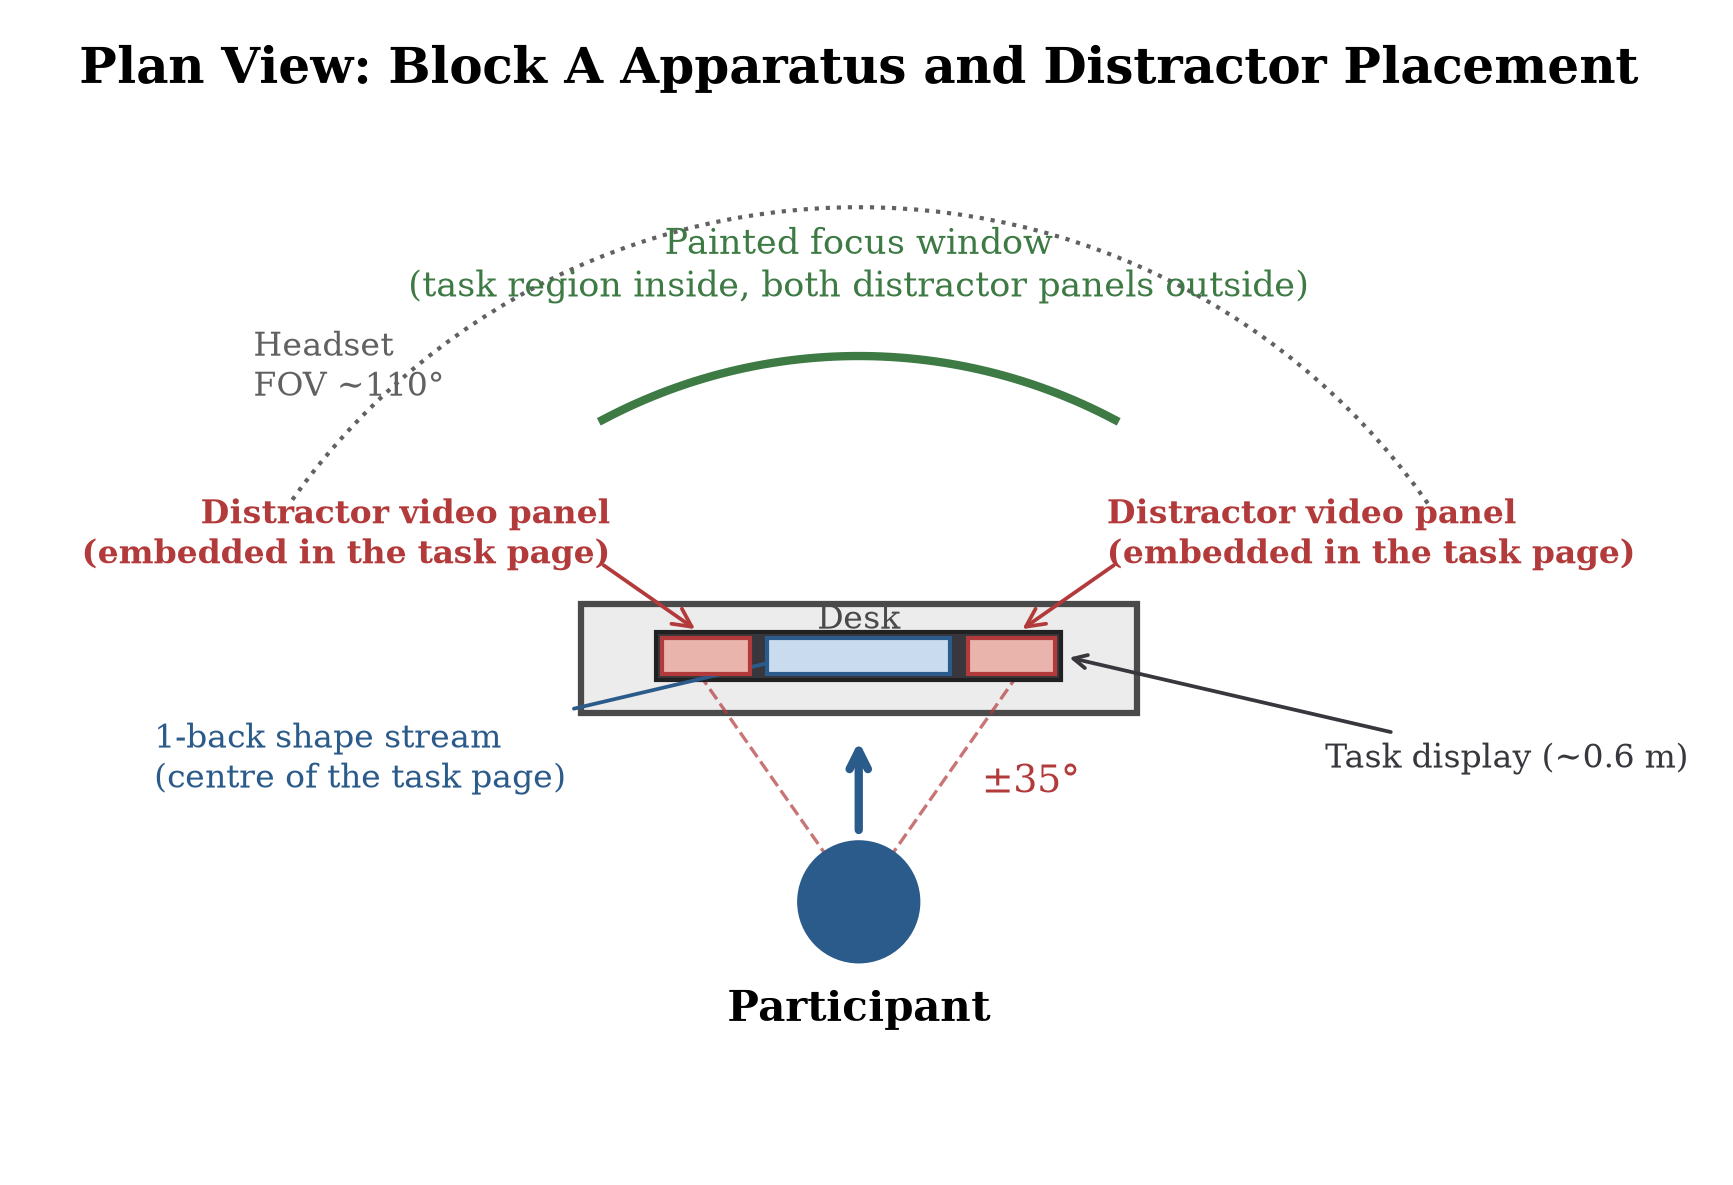
\includegraphics[width=0.78\linewidth]{content/figures/fig_block_a_layout.png}
\caption{Plan view of the Block A apparatus and distractor placement.}
\label{fig:blockalayout}
\end{figure}

The two conditions are \textbf{NoFilter}, where the window is painted but invisible, and
\textbf{Filter}, Hard Dark on. In the final task version each lasts 4 minutes 40 seconds, which is
140 trials at a 2.0 s stimulus onset asynchrony, run once each per participant in counterbalanced
order. Earlier sessions ran shorter versions of the same task (Section 5.7). Before the first
condition the participant paints the focus window around the central task region and releases to
lock it, and the experimenter verifies that both distractor panels fall outside it and the entire
task region inside. The same locked window persists across both conditions. Hard Dark's job here is
to occlude the distractor panels from view entirely, not merely dim them at a distance.

\textbf{The task is a forced-choice 1-back.} The centre of the task display, inside the focus
window, presents one look-alike shape at a time, drawn from a set of six at $\geq$ 3$^{\circ}$
visual angle, and the participant answers yes or no on every shape to ``same as the previous shape?''
via trigger press. Two choices in that sentence are load-bearing. The task is seen through the
window's untouched native passthrough and its shapes are deliberately large, because Quest 3
passthrough does not reach normal visual acuity and a task requiring fine detail would floor out in
every condition for reasons unrelated to the vignette; the shape stream's legibility through
passthrough is a pilot gate (Appendix A, gate G1), not an assumption. And it is forced-choice
rather than Go/No-go, because a Go/No-go stream ceilinged out at
96--100\% accuracy in piloting regardless of condition, which would leave the block unable to detect
any vignette effect at all. The 1-back adds a working-memory component on top of the reactive one,
and its memoryless 50\%-repeat sequence keeps performance off ceiling.

Error rate, the primary dependent variable, is misses plus commissions, logged to the millisecond. No
per-trial correctness feedback is given during scored runs, only pacing feedback, so feedback cannot
shift a participant's speed-accuracy strategy mid-run. The window uses room-geometry anchoring for
this block specifically rather than the direction-lock used by default, so four corner rays captured
on release are remembered as physical points and the window stays put as the participant leans toward
or away from the desk. Head-turns toward the distractor panels beyond 30$^{\circ}$ yaw are recorded
from 60 Hz telemetry as an exploratory measure.

\section{Block B: Secondary, Driving Marker Detection}

The comparison is again Filter against NoFilter, and the task uses the driving footage's own content
as the target. A ring marker is authored onto each real traffic-light or pedestrian object as it
appears, and the participant presses the trigger on noticing it. Putting the target on a real object
rather than on an abstract probe overlaid on the scene is what makes the measurement direct: the
object under the marker is exactly the kind of object SignPop's detection gate is built to reveal.

Both conditions play the same clip in full, running 8 minutes 39 seconds each, so the two differ only
in shader state and in which marker set is scored. The focus window is pre-set to the windscreen
region and direction-locked for all participants, so the guided region stays constant across the
sample. Condition order alternates by participant parity, and the two marker sets are alternated
against condition so neither set is systematically tied to Filter or NoFilter.

\textbf{Forty scored markers per condition, drawn from two disjoint sets of forty over the same
clip}, which is 1,200 marker presentations across the fifteen usable pairs. Using a different set in
each condition stops a participant meeting the same target twice, which would turn the second
condition into a memory test. Each marker fades in rather than switching on, because sudden onsets
capture attention automatically and would swamp the effect being measured \citep{yantis1984}, and it
modulates the pixels underneath rather than covering them, so it keeps its own internal contrast even
where the filter has dimmed everything under it \citep{wallis2015}. \textbf{The marker itself is
dimmed by the same falloff as the rest of the scene regardless of condition, so a filtered marker is
never easier to see as a marker.} Only the object beneath a detected marker is treated differently
between conditions. Seventy of the eighty authored targets fall inside an active detection window
while on screen. Figure~\ref{fig:ring} shows the marker's construction, rendered directly from the
shader's arithmetic at the study's parameters.

\begin{figure}[htbp]
\centering
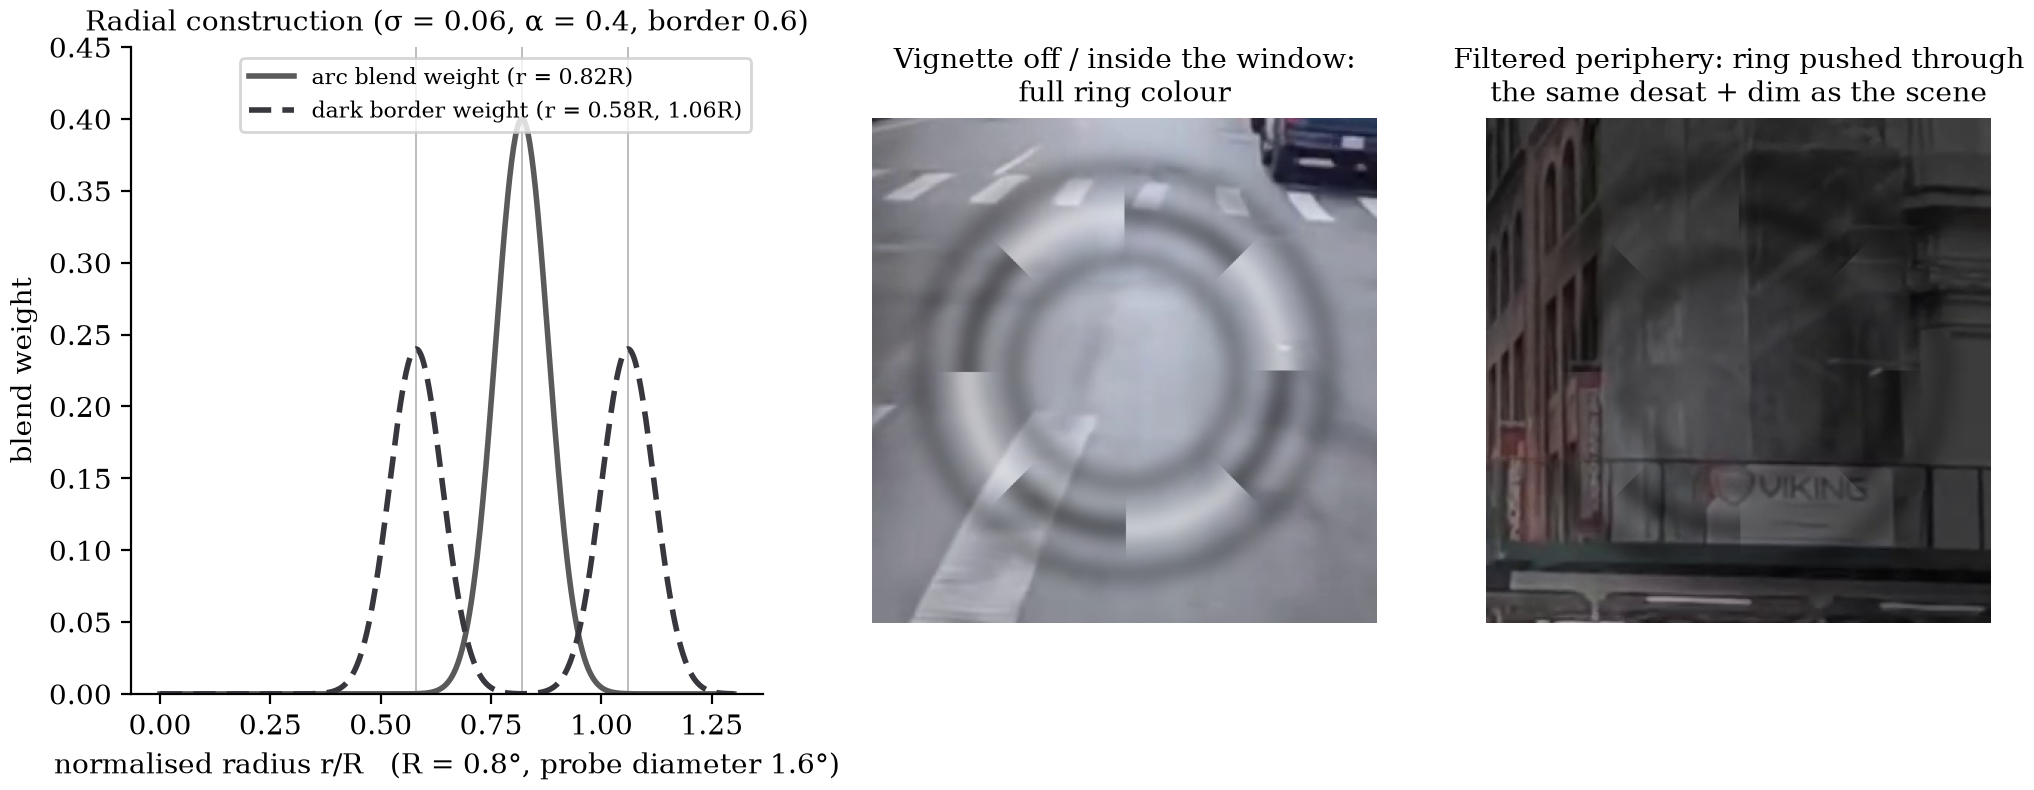
\includegraphics[width=\linewidth]{content/figures/fig_ring_probe.png}
\caption{The ring marker, constructed from the shader's own arithmetic at the study configuration
and shown enlarged (the probe subtends 1.6\textdegree{} in the headset). The marker is a translucent
``rope'': four alternating black-and-white arc pairs on a Gaussian annulus at 0.82 of the probe
radius (40\% opacity), flanked by two multiplicative dark borders. The pattern is achromatic, so the
filter's desaturation cannot erase it, and its polarity alternates, so some arc contrasts with any
background it lands on. The marker fades in over 0.5 s rather than onsetting abruptly
\citep{yantis1984}. Centre and right: the same marker over an unfiltered and a filtered region of
the driving scene. The borders darken multiplicatively and the white arcs are pushed through the
same desaturation and dim the grading applies to the scene at that pixel, so the pattern's internal
contrast survives while the marker as a whole dims like a real object rather than advertising
itself \citep{wallis2015}.}
\label{fig:ring}
\end{figure}

A \textbf{hit} is a trigger press while the marker is on screen, within 10$^{\circ}$ of its position
at that instant. Presses landing on nothing are false alarms. Markers move while visible, by
17$^{\circ}$ of travel on average, so scoring against a marker's average position misassigns a
meaningful share of presses to the wrong analysis band. The intended method is therefore to score
every press against the marker's reconstructed position, from the recorded scene track, at the exact
instant of the press. That reconstruction is not yet implemented in the analysis pipeline, so the
band table reported in Section 5.7.3 assigns each target by its mid-lifetime position instead, and
the size of the resulting misassignment is stated there as a limit on the band finding.

\textbf{Eccentricity bands.} Each scored marker is assigned to one of four bands, fixed from
published gaze landmarks before any data was seen. Driver gaze concentrates in a road-centre region
of roughly 8$^{\circ}$ radius \citep{victor2005}, so the under-10$^{\circ}$ band covers what a viewer
is looking at anyway. The Peripheral Detection Task, the standard instrument for measuring spare
attentional capacity under load, places its probes just outside that region at 11--23$^{\circ}$
horizontal eccentricity \citep{jahn2005}, and the Detection Response Task standardises the same logic
with a fixed, background-independent stimulus \citep{iso2016}. The 10--20$^{\circ}$ and
20--30$^{\circ}$ bands bracket that published range. The outer boundary is the conventional
useful-field extent of roughly 30$^{\circ}$ \citep{ball1993}, past which a stronger peripheral signal
has little left to buy. One point of fit is worth stating precisely, because the 20--30$^{\circ}$
band carries H2a: the published probe range stops at 23$^{\circ}$, so it covers 10--20$^{\circ}$
completely but only the lower part of 20--30$^{\circ}$. The boundaries bracket the published
landmarks rather than reproducing any one study's geometry.

Figure~\ref{fig:bandlandmarks} places the four bands against the published landmarks they were
drawn to bracket.

\begin{figure}[htbp]
\centering
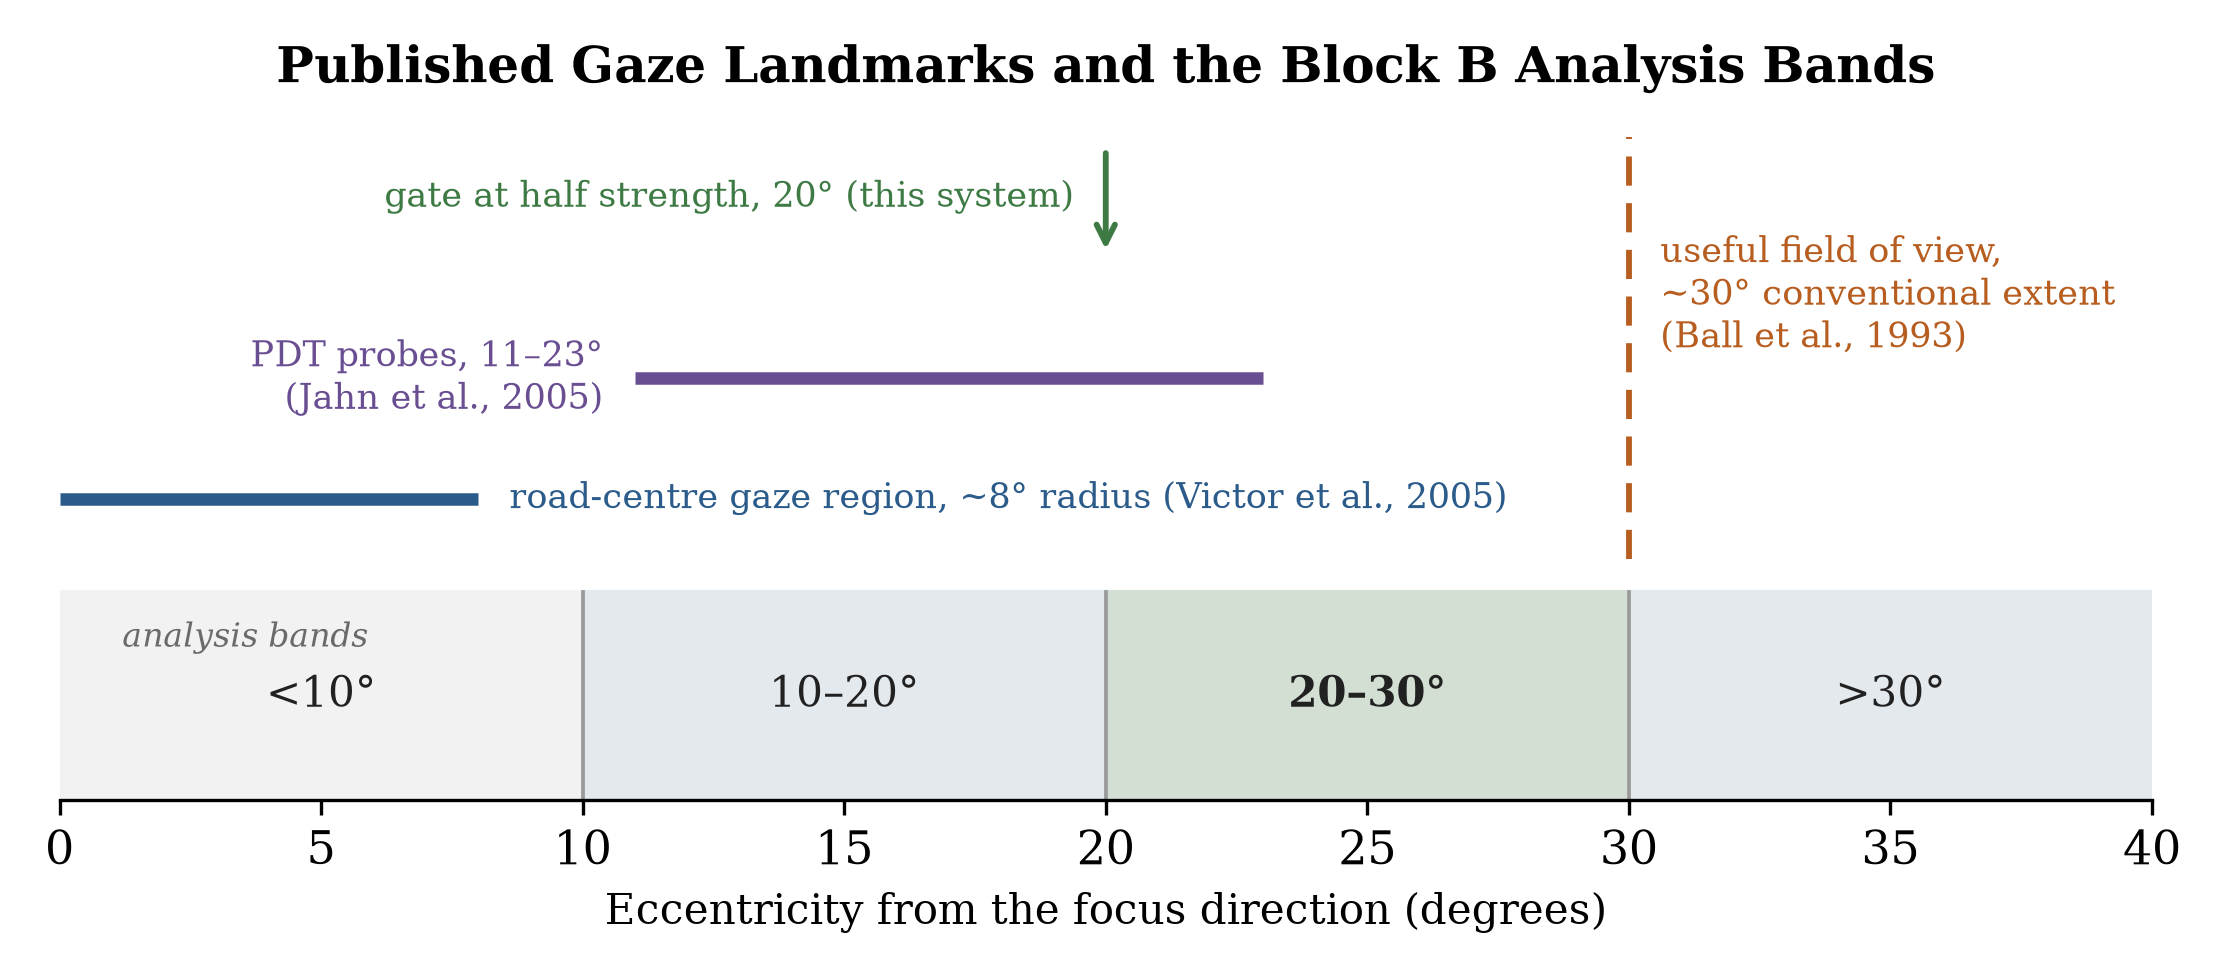
\includegraphics[width=\linewidth]{content/figures/fig_band_landmarks.png}
\caption{The four Block B analysis bands against the published gaze landmarks that fixed their
boundaries: the road-centre gaze region \citep{victor2005}, the Peripheral Detection Task probe
range \citep{jahn2005}, the conventional useful-field extent \citep{ball1993}, and the system's own
soft edge at 20\textdegree{}. The published probe range stops at 23\textdegree{}, so the
20--30\textdegree{} band is only partly covered by it.}
\label{fig:bandlandmarks}
\end{figure}

Head pose serves as the attention proxy in place of eye tracking, which the Quest 3 does not provide.
Head orientation is a validated gaze surrogate at the eccentricities used here
\citep{higgins2022,sitzmann2018}.

\section{Block C, and What It Cost to Cut}

Block C answers RQ3 and carries no confirmatory claims. A three-mode sampler was specified here, 75
seconds each of SignPop, Soft Dark and Hard Dark on common footage, and \textbf{it was cut from the
running protocol} because the two confirmatory blocks already account for roughly 35 minutes in the
headset and the sampler would have added two further exposures at the point of maximum fatigue. Two
consequences follow and are carried through this dissertation rather than absorbed quietly. Soft Dark
was never shown to a participant, so no participant data on it exists (Chapter 3, Section 3.4). And
no participant ever saw two modes on a common stimulus, so Hard Dark is tested only at the
workstation and SignPop only in the driving scene. Every confirmatory claim here is therefore a
\textit{mode-in-context} claim, never a mode-generalised one, and nothing in the design softens that
confound.

The instrument is a single end-of-session questionnaire, self-completed with the headset off after
the post-session sickness questionnaire and before the debrief, so opinions are captured before the
hypotheses are revealed. It carries 21 rated items across four sections, plus a preference ranking
and a multi-select. The three scored constructs, perceived focus benefit, perceived awareness cost
and visual comfort, carry 15 of those items, each mixing positively and negatively keyed items to
counter acquiescence bias. The fourth section, on acceptance and willingness to use, was not
administered, so the study has no acceptance data. Because it asks for one considered opinion of the whole session, it cannot
separate Hard Dark's contribution from SignPop's. It is a system-level instrument, reported as
exploratory.

\section{Results}

Eighteen people were tested. The pre-registered target was twenty, and collection ended two short of
it when the dissertation deadline arrived. That shortfall is a protocol deviation, and the status
note at the head of this chapter reports it as one. The analysis proceeds on a specific ground rather than convenience: the 20-participant
target existed to buy 80\% power for the primary contrast, and the achieved sample already delivers
it, at 82\% for the primary contrast and 84\% for the pre-registered eccentricity band (both
one-tailed, matched to the directional hypotheses). What the shortfall does cost is stated where it
binds: the pooled Block B estimate remains underpowered, and every confidence interval below is two
participants wider than the design intended.

Block A yields \textbf{seventeen} usable paired participants and Block B \textbf{fifteen}, the two sets
overlapping but not identical because some participants contributed a usable result to one block and
not the other. One participant is excluded from Block A: P1's task rounds ran about fifteen minutes
after the session's Unity blocks closed, so the arm assignment cannot be verified from the session
ledger. That exclusion is specific to Block A, and P1's Block B pair is unaffected and is analysed.
Three participants are excluded from Block B under documented rules, never inferred ones. Two fall
under the pre-registered response-validity rule: P3 for 539 false alarms on the filter run with
provably looser hits (Mann-Whitney $p = .0301$), and P43 for false-alarm counts of 81 and 54 across
the two arms, the highest in the set by a wide margin, on the same grounds as P3. The third is P9,
excluded by experimenter decision on the day under the task-comprehension rule: the response rule
was not yet understood during that participant's first video block, which was their first exposure
to the task. Separately, P15 and P16 are two ledger IDs for one participant, reconciled into a
single record under the relaunch rule of Appendix~A, Section~A.4. That participant's P15 Block B run
is excluded for 206 false alarms across 246 presses, so the P16 pair is their Block B record and the
P15 pair their Block A record.
Block A is retained for P3, P9 and P43, since those exclusions concern the marker task alone. The
arithmetic closes on the eighteen tested: seventeen contribute a Block A pair, the eighteen less P1,
and fifteen contribute a Block B pair, the eighteen less P3, P9 and P43.

Two provenance facts belong with the numbers rather than in a footnote. Block A pools four versions
of the same task. The first five participants ran a short version of 84 or 105 trials that sat at
95.2\% mean accuracy, and everyone from P9 onward ran the 140-trial version, which was changed
deliberately to move performance off that ceiling. Pooling is justified by the robustness split
reported below, where the two halves of the sample return the same effect at the same size. And one
of the thirty-four Block A arms, P4's filter-off arm, is the experimenter's contemporaneous record
rather than an exported
file, which is why the trial count in Section 5.1 is given as file-backed. Dropping that arm changes
nothing ($p = .0175$ against $.0212$, $d_z$ unchanged).

\subsection{H1: workstation focus}

\textbf{The pre-registered primary test.} Table~A.4 registers H1's primary test as a trial-level
logistic model with a participant random effect, and the paired test as its robustness
check. Across the 4,125 file-backed scored trials from seventeen participants the vignette term is
significant: \textbf{odds ratio 0.583} (95\% CI 0.396 to 0.860, $z = -2.724$, $p = .0065$), so Hard
Dark \textbf{reduces trial-level error odds by 41.7\%}. The estimator fitted is a logistic GEE with
an exchangeable working correlation clustered by participant, because statsmodels offers no strict
frequentist mixed model with p-values, a substitution already documented in
\texttt{Tools/analysis/h1\_lmm.py}. The literal random-intercept specification agrees, at odds
ratio 0.578 with a 95\% credible interval of 0.474 to 0.704. Trial-level models use 33 of the 34
Block A arms, because P4's filter-off arm has no exported file. The robustness check agrees in
direction and significance, and is the weaker of the two because it averages within participants
before testing rather than using the trials themselves.

\textbf{The registered robustness check.} Accuracy on the memory task rose from 92.30\% (SD 6.56) with the vignette off to 95.39\% (SD 4.17)
with Hard Dark on. That is a gain of \textbf{+3.09 percentage points} (SD 4.79, median +2.16; 95\% CI
+0.62 to +5.55, paired $t(16) = 2.66$, $p = .017$; Wilcoxon $W = 21.0$, $p = .015$; $d_z = 0.645$).
Twelve of seventeen participants improved, four declined, one was unchanged. Achieved power at this
sample and effect size is 82\% one-tailed, so the sample delivers the power level the design chose
its 20-participant target to provide.

\textbf{H1's direction is confirmed; its pre-set size is not, and the decision table is applied as
written.} Both the parametric and the rank test agree, the rank test, the more conservative of the
two here, returns the lower p-value, so the result does not depend on the normality assumption, and
the refuting observation, a difference absent, reversed, or with its 90\% interval excluding the
smallest effect size of interest from below, did not occur. But the hypothesis asked for more than a
direction. Its default smallest effect size of interest was half of the vignette-off error rate,
which at the achieved data is 3.85 of 7.70 points, and the observed reduction is 3.09 points, 40\%
of the distractor-laden error rate, with a 90\% interval from 1.06 to 5.12 that spans the 3.85-point
mark. That is row 4 of the pre-committed decision table: \textit{the benefit is real-signed but
cannot be claimed at the pre-set size}. The bounded conclusion the table prescribes is therefore the
claim: Hard Dark removes between roughly 14\% and 66\% of the error rate that distractor-laden work
carries (90\% CI), with 40\% the best estimate, a real benefit that falls short of certainty at the
half-the-errors bar the design set itself.

The estimate itself is stable. It barely moved as the sample grew, from +3.34 at
fourteen pairs to +3.09 at seventeen, which is what a real but modest effect looks like under
accumulation. One robustness split deserves stating rather than burying: the first five participants
ran a shorter task version and the remaining twelve ran the 140-trial version, and the two groups
give the same effect at the same size, +3.30 and +2.99 points. What differs is spread (SD 2.30
against 6.10), because the early task sat near ceiling and compressed every delta, while the harder
version moved performance off ceiling at the cost of individual variation. Pooling therefore
combines two measurements of one effect rather than two different effects.
Figure~\ref{fig:h1} shows every participant's pair.

\begin{figure}[htbp]
\centering
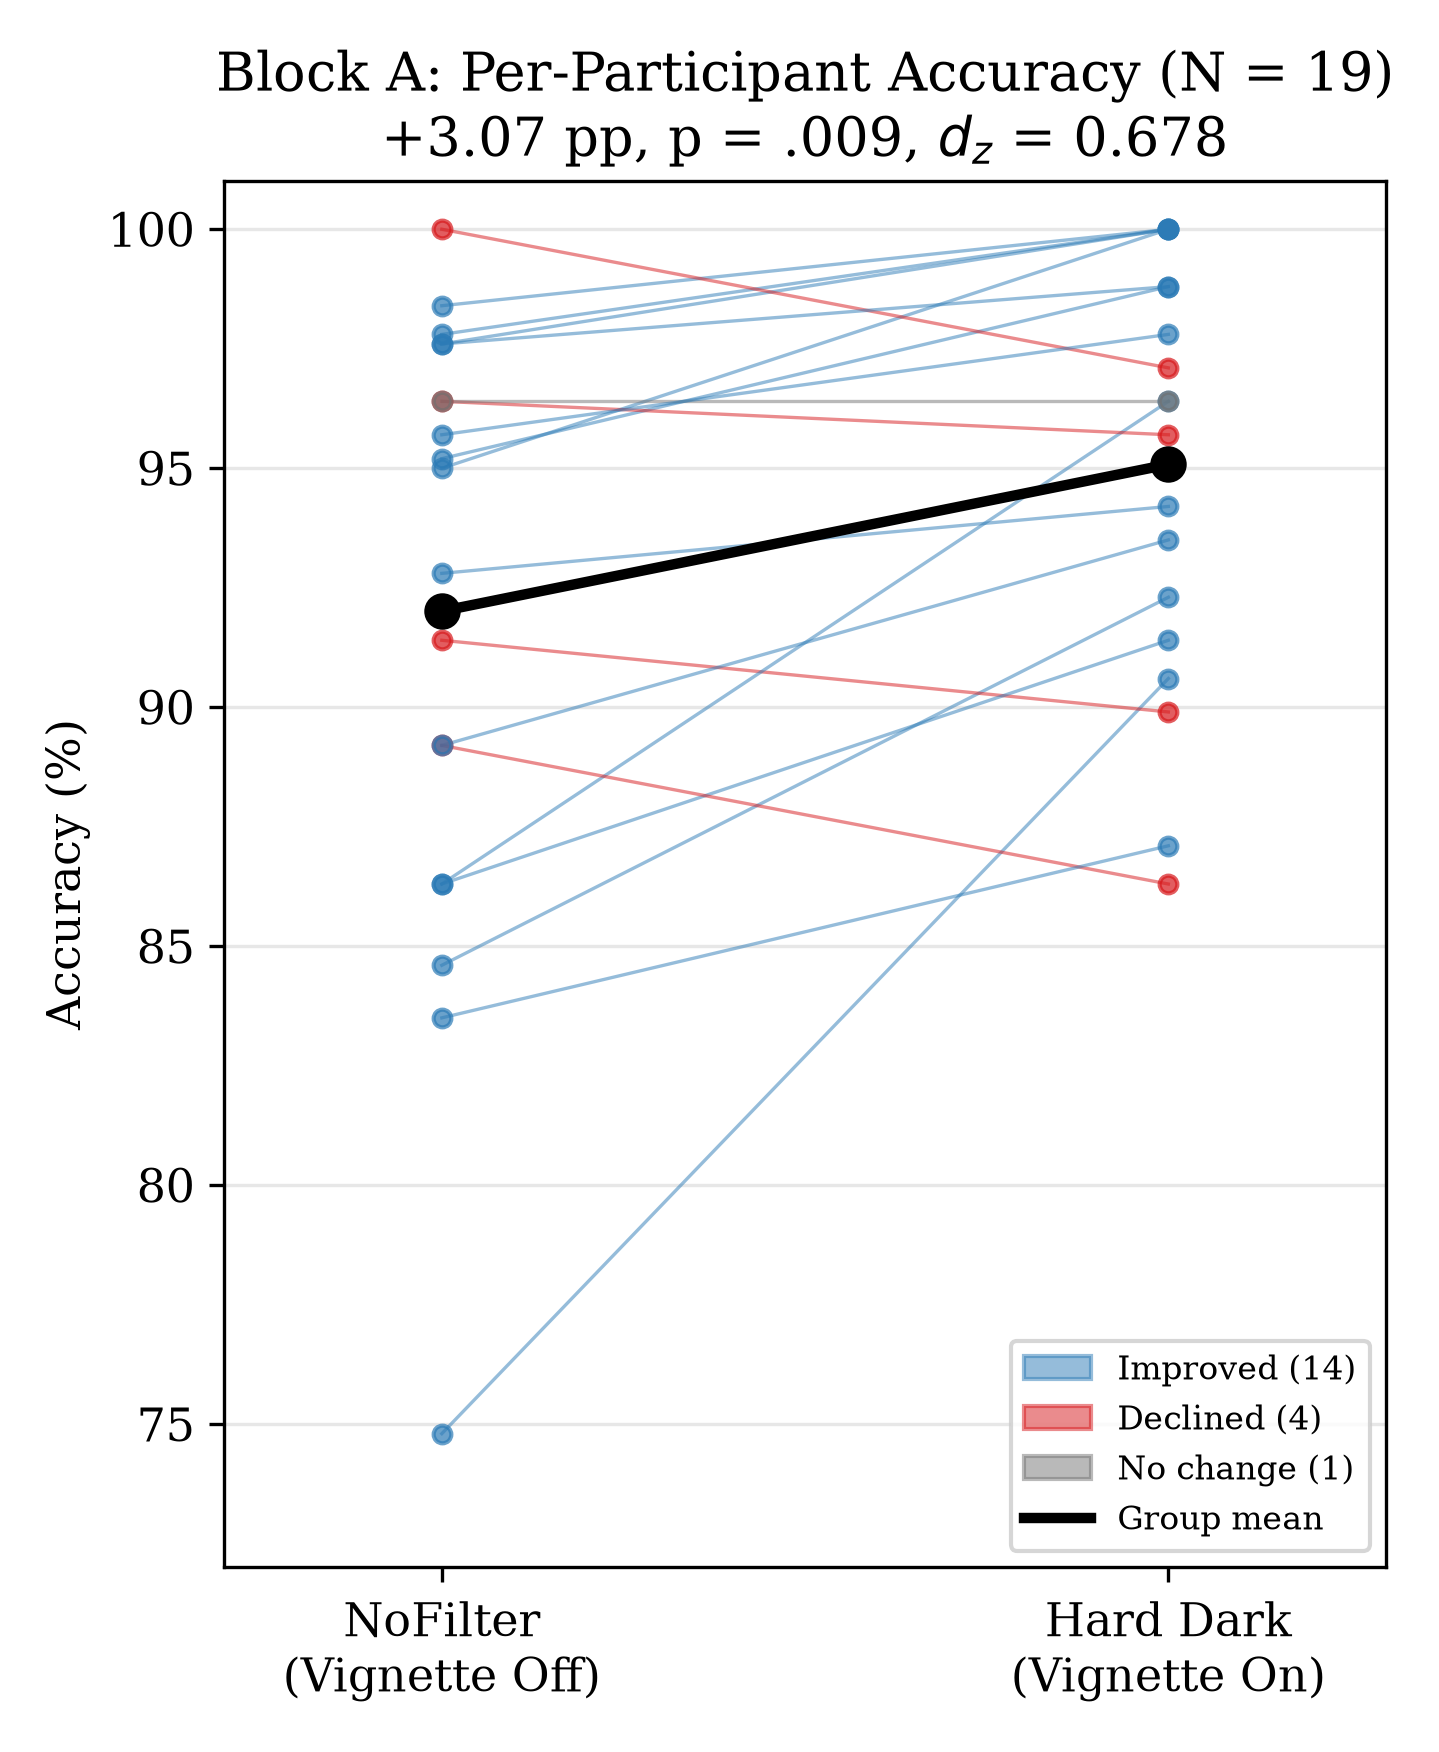
\includegraphics[width=\linewidth]{content/figures/fig_slopegraph_h1.png}
\caption{Block A per-participant accuracy, vignette off versus Hard Dark on (N = 17).}
\label{fig:h1}
\end{figure}

\subsection{H2b: the pooled safety check}

Hit rate pooled across the whole field of view rose by \textbf{+6.00 percentage points} with SignPop
on, from 50.67\% (SD 16.54) to 56.67\% (SD 8.85), with eight of fifteen participants improving. The
paired difference test does not reach significance ($t(14) = 1.74$, $p = .105$; Wilcoxon $W = 27.0$,
$p = .109$), which is beside the point, because H2b was never a difference test.

\textbf{H2b's refuting observation did not occur, so the safety claim stands.} Section 5.2 committed
in advance to what would refute H2b: equivalence not established \textit{and} a point estimate
showing a drop greater than 10 points. The estimate is a rise of 6.00 points, so the second condition
is not met and the mode is not shown to harm situational awareness. The 90\% confidence interval runs
$-0.09$ to $+12.09$, so the worst case the data support is no loss at all to within a tenth of a
point, far inside the ten-point margin.

\textbf{The pre-registered statistic is nonetheless worth reporting exactly.} The two one-sided
tests return $p = .0002$ on the lower bound and $p = .133$ on the upper, so formal equivalence within
$\pm$10 points is not established at this sample. The reason is entirely one-directional: the data
cannot exclude a \textit{benefit} larger than ten points. That is a specification issue rather than a
result. H2b asks a one-sided question, whether re-grading costs peripheral awareness, and a two-sided
procedure additionally requires ruling out a large gain, which the safety framing never cared about.
The instrument matched to the question is a non-inferiority test against a $-10$-point margin, which
is the lower one-sided test above, and it passes decisively. Both numbers are given so the reader can
see the pre-registered procedure and the question it was meant to serve. What this dissertation does
not do is quietly substitute the better-fitting reading for the pre-registered one after seeing the
data. A study writing a safety bound should state the direction it cares about and test that
direction alone.
One adjacent observation does not help and is reported anyway: false alarms rose under the filter,
a mean of 12.7 presses per run against 7.3 with it off, with nine of fifteen participants pressing
more. Hit rate does not correct for response criterion, so part of the pooled rise may be a more
liberal response strategy rather than better detection. The exclusion rule bounds the worst of this
(P43's counts were double the next participant's and are excluded), and the band analysis below is
unaffected in kind, but the pooled estimate carries this qualification.
Figure~\ref{fig:h2b} places the estimate against the margin.

\begin{figure}[htbp]
\centering
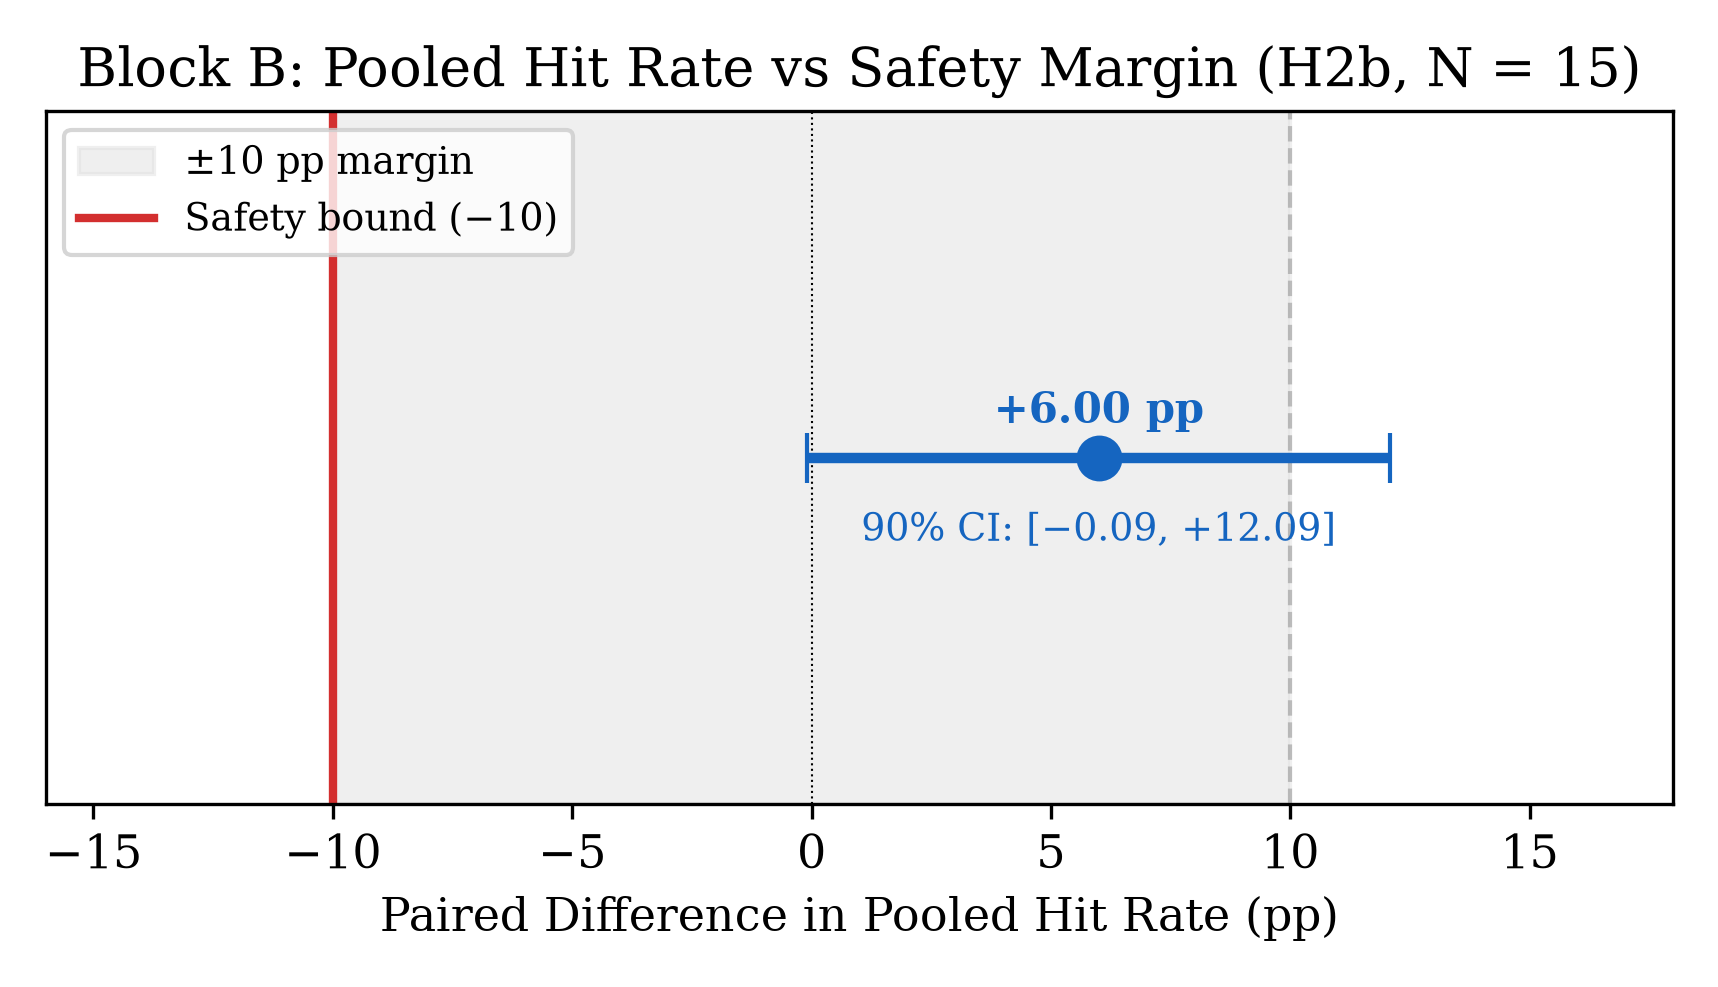
\includegraphics[width=\linewidth]{content/figures/fig_equivalence_h2b.png}
\caption{Block B pooled hit rate against the safety margin (H2b, N = 15).}
\label{fig:h2b}
\end{figure}

\subsection{H2a: the 20--30\textdegree{} band}

Hit rate broken out by eccentricity band, in Table~\ref{tab:bands}, shows a pattern rather than a
uniform shift. Every band moves in the same direction, but only one moves reliably.

Two estimators are reported because they answer different questions and, in one band, disagree. The
\textbf{pooled} rate weights every marker presentation equally and is what the bars of
Figure~\ref{fig:h2a} show. The \textbf{per-participant} mean weights every participant equally, and
it is the estimator the paired tests and confidence intervals belong to. Participants contribute
unequal numbers of markers to a band, so the two can differ, and in the under-10$^{\circ}$ band they
differ in sign.

\begin{longtable}{p{0.13\textwidth}|p{0.16\textwidth}|p{0.16\textwidth}|p{0.17\textwidth}|p{0.20\textwidth}}
\caption{Block B hit rate by eccentricity band. Pooled rates weight every marker presentation
equally; the difference column and its interval are per-participant, which is what the tests use.}
\label{tab:bands} \\
\hline
\textbf{Band} & \textbf{Off, pooled} & \textbf{On, pooled} & \textbf{Difference (per participant)} & \textbf{90\% CI, $p$} \\
\hline
\endfirsthead
\hline
\textbf{Band} & \textbf{Off, pooled} & \textbf{On, pooled} & \textbf{Difference (per participant)} & \textbf{90\% CI, $p$} \\
\hline
\endhead
\hline
$<$10\textdegree{} & 75.0\% & 79.8\% & $-2.50$ pp & $[-11.7, +6.7]$, $p = .638$ \\
10--20\textdegree{} & 41.5\% & 47.9\% & $+6.77$ pp & $[-3.8, +17.3]$, $p = .278$ \\
\textbf{20--30\textdegree{}} & \textbf{40.2\%} & \textbf{57.7\%} & \textbf{$+17.78$ pp} & \textbf{$[+6.6, +29.0]$, $p = .014$} \\
$>$30\textdegree{} & 55.0\% & 55.6\% & $+0.56$ pp & $[-6.8, +7.9]$, $p = .896$ \\
\hline
\end{longtable}

\textbf{H2a is supported, in the band it was pre-registered on.} The
20--30$^{\circ}$ band is the only one whose interval excludes zero, so its refuting observation did
not occur, and it is roughly three times larger than any other band ($d_z = 0.72$, Wilcoxon
$p = .021$, achieved power 84\% one-tailed). It is the one Block B measure that is both significant
and adequately powered at this sample.

What makes it more than a lucky slice is that the band was fixed by the system's geometry before any
data existed. The soft edge was set at 20$^{\circ}$ against the useful field of view, and the benefit
appears in precisely the annulus between where the gate starts having room to act and where the
useful field runs out. Inside 20$^{\circ}$ the gate has nothing to reveal, and beyond 30$^{\circ}$ it
reveals plenty to an eye that can no longer use it. This is a prediction from the shader agreeing
with the data rather than a pattern fitted to it afterwards.

Two limits belong beside the finding. Band membership in this table uses each target's mid-lifetime
position, which is a weak proxy: targets move, the median lifetime swing is 17.2$^{\circ}$, and
roughly 31\% of catches land in a different band from the one the mid position assigns. And with the
pooled rate rising in every band while the inner band is near ceiling in both conditions, the honest
reading is a general positive trend with one band carrying almost all of the signal, rather than
three null bands and one live one.

\begin{figure}[htbp]
\centering
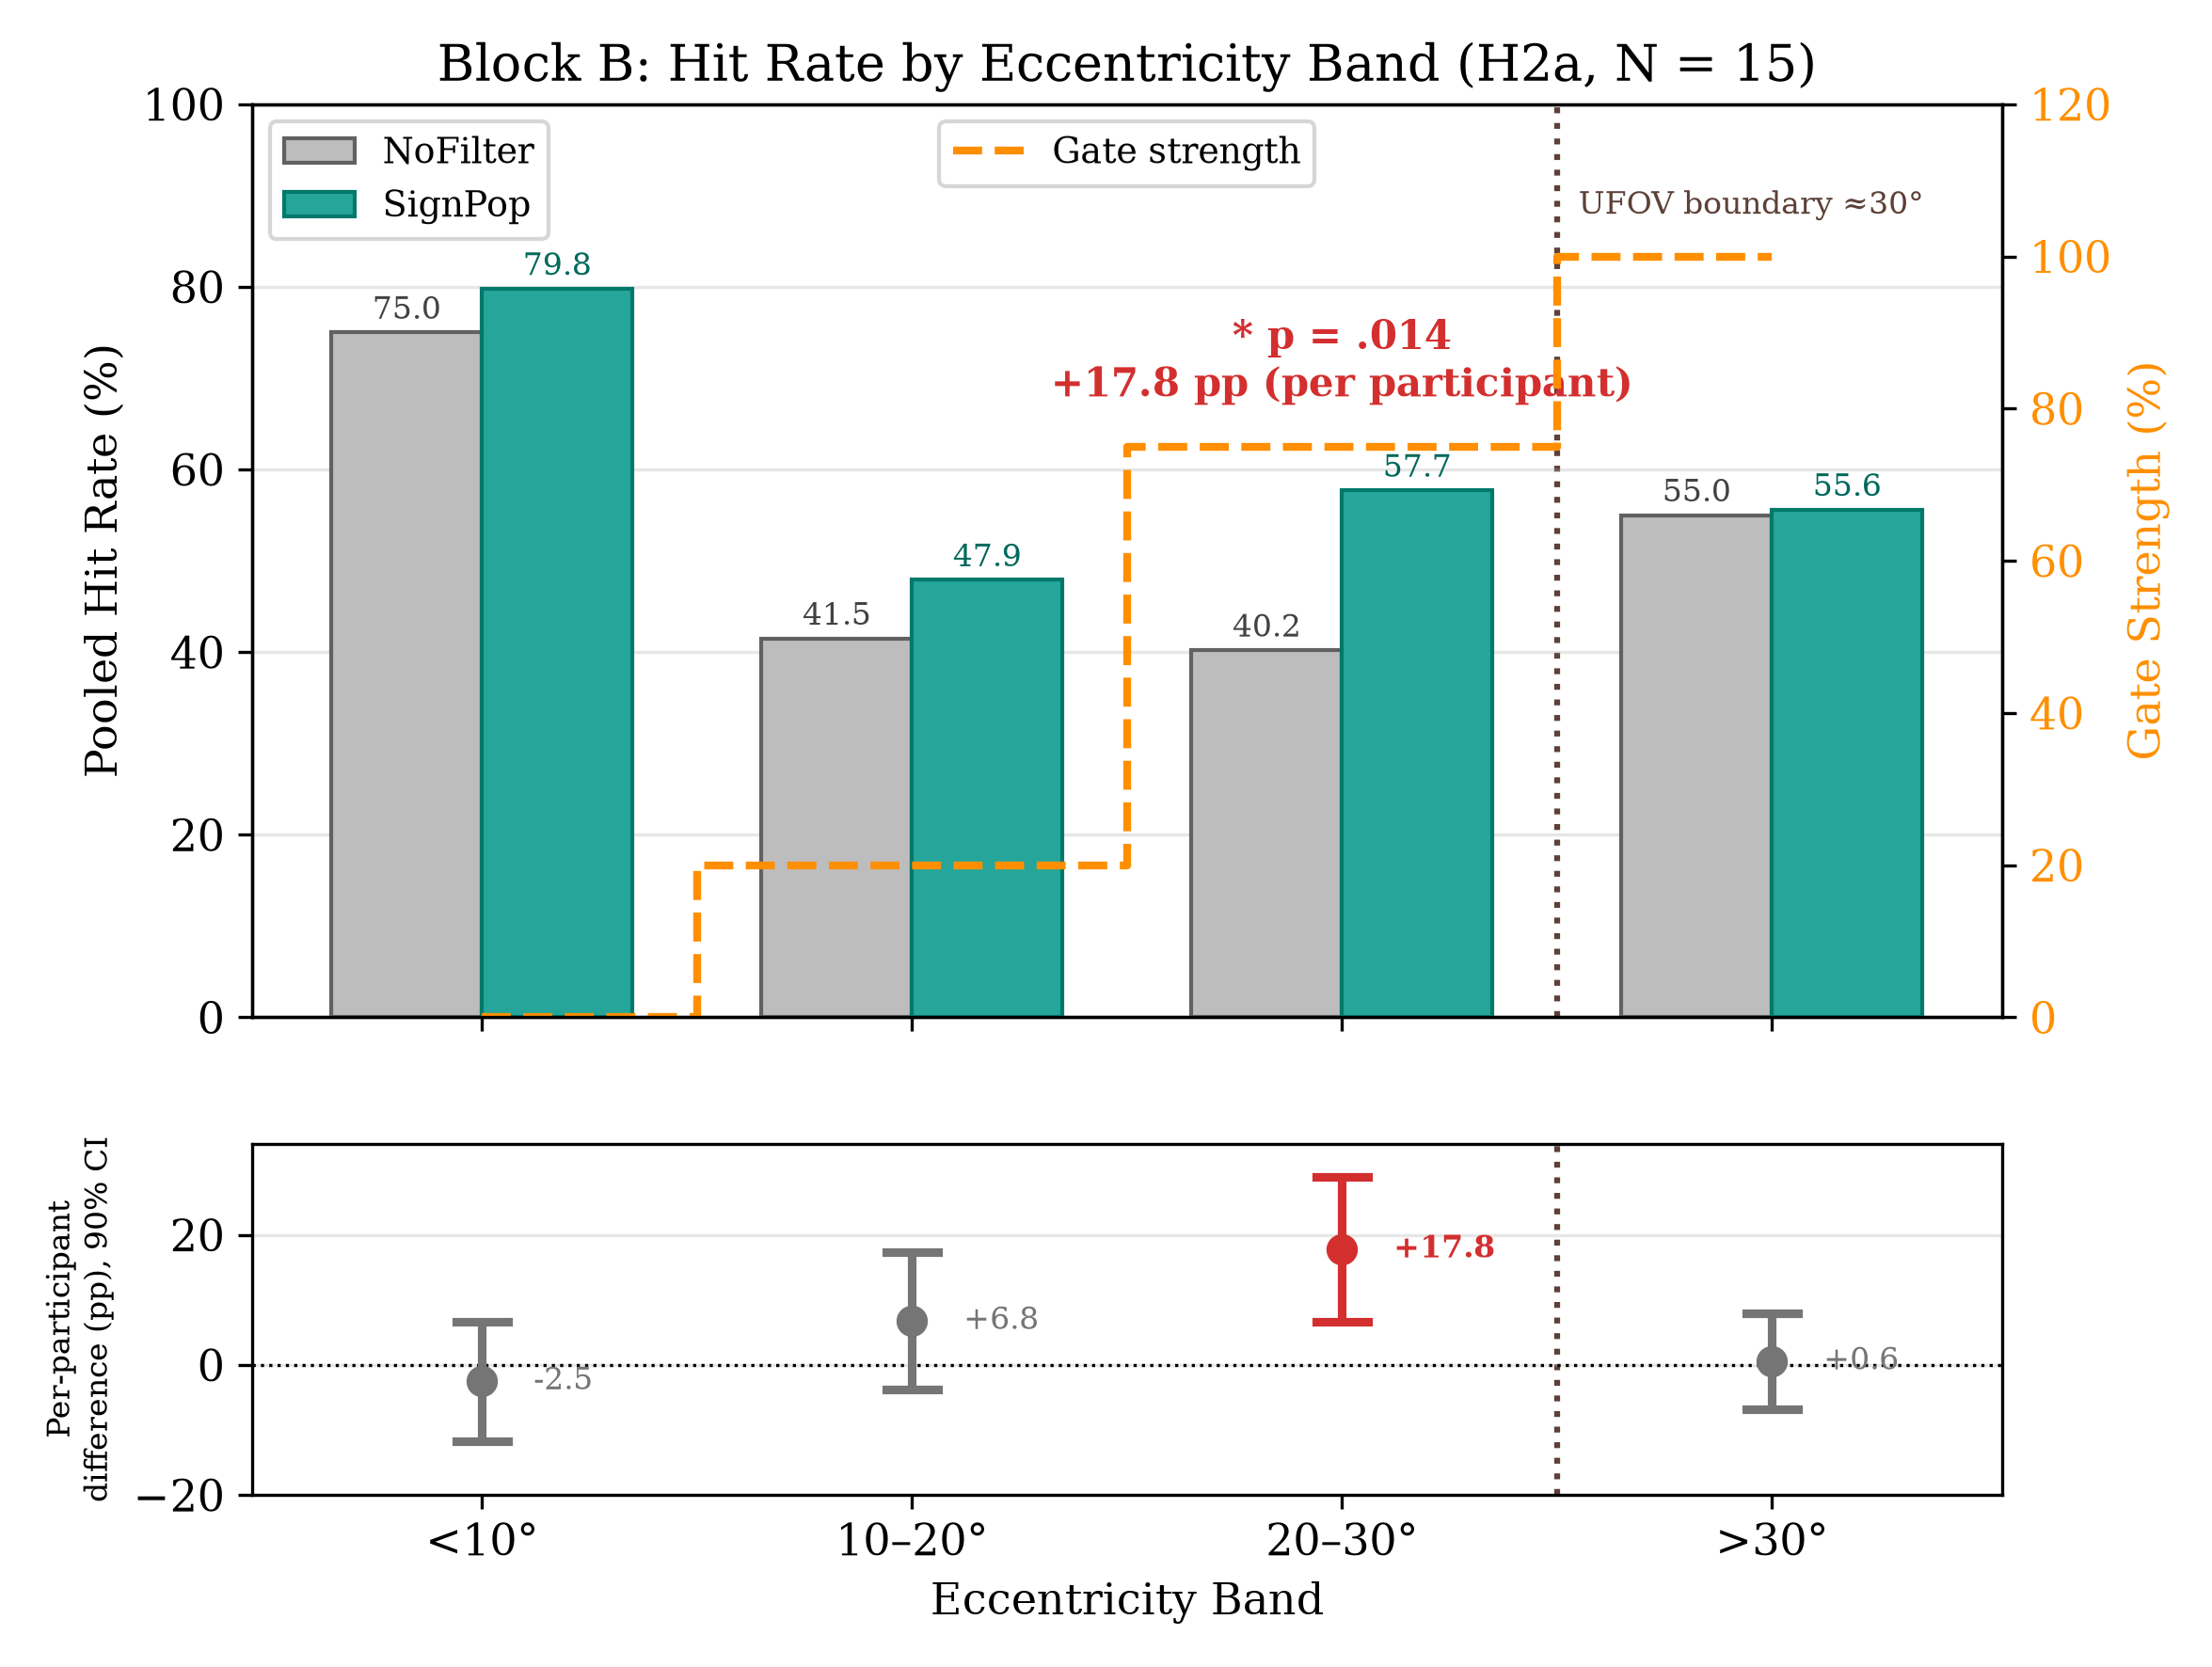
\includegraphics[width=\linewidth]{content/figures/fig_eccentricity_h2a.png}
\caption{Block B hit rate by eccentricity band, with gate strength and the useful-field boundary
overlaid (H2a, N = 15). The upper panel pools every marker presentation in a band. The lower panel
gives the paired per-participant difference with its 90\% interval, which is the estimator the tests
use, and which for the $<$10\textdegree{} band differs in sign from the pooled figure because
participants contribute unequal numbers of markers to a band.}
\label{fig:h2a}
\end{figure}

\subsection{What participants said, and where it disagrees}

Sixteen end-of-session questionnaires show a divergence worth flagging rather than resolving.
Perceived focus benefit is strongly positive, 71 of 80 responses favouring the effects. Perceived
awareness cost splits close to evenly at 46 of 80, so roughly four in ten responses report feeling
cut off from the surroundings or noticing side events late. The split is item-shaped rather than
person-shaped: ``I still felt aware of my surroundings'' runs 13 of 16 in the filter's favour, while
``I noticed side events later than I would have'' and ``I was comfortable not seeing everything''
each run 7 of 16. Visual comfort sits at 45 of 64 across its four answered items. The focus-benefit
items on holding attention, looking away and knowing where to look were answered favourably by 15,
14 and 15 of the sixteen respondents. At the earlier ten-participant analysis these three were
unanimous and they no longer are, which is a useful reminder of how little weight a unanimous result
at that sample size could carry. One respondent dissents strongly across the focus-benefit block,
answering one of its five items favourably, so the construct is not uniformly endorsed even where it
is strongest. Figure~\ref{fig:esq} shows the three constructs side by side.

\begin{figure}[htbp]
\centering
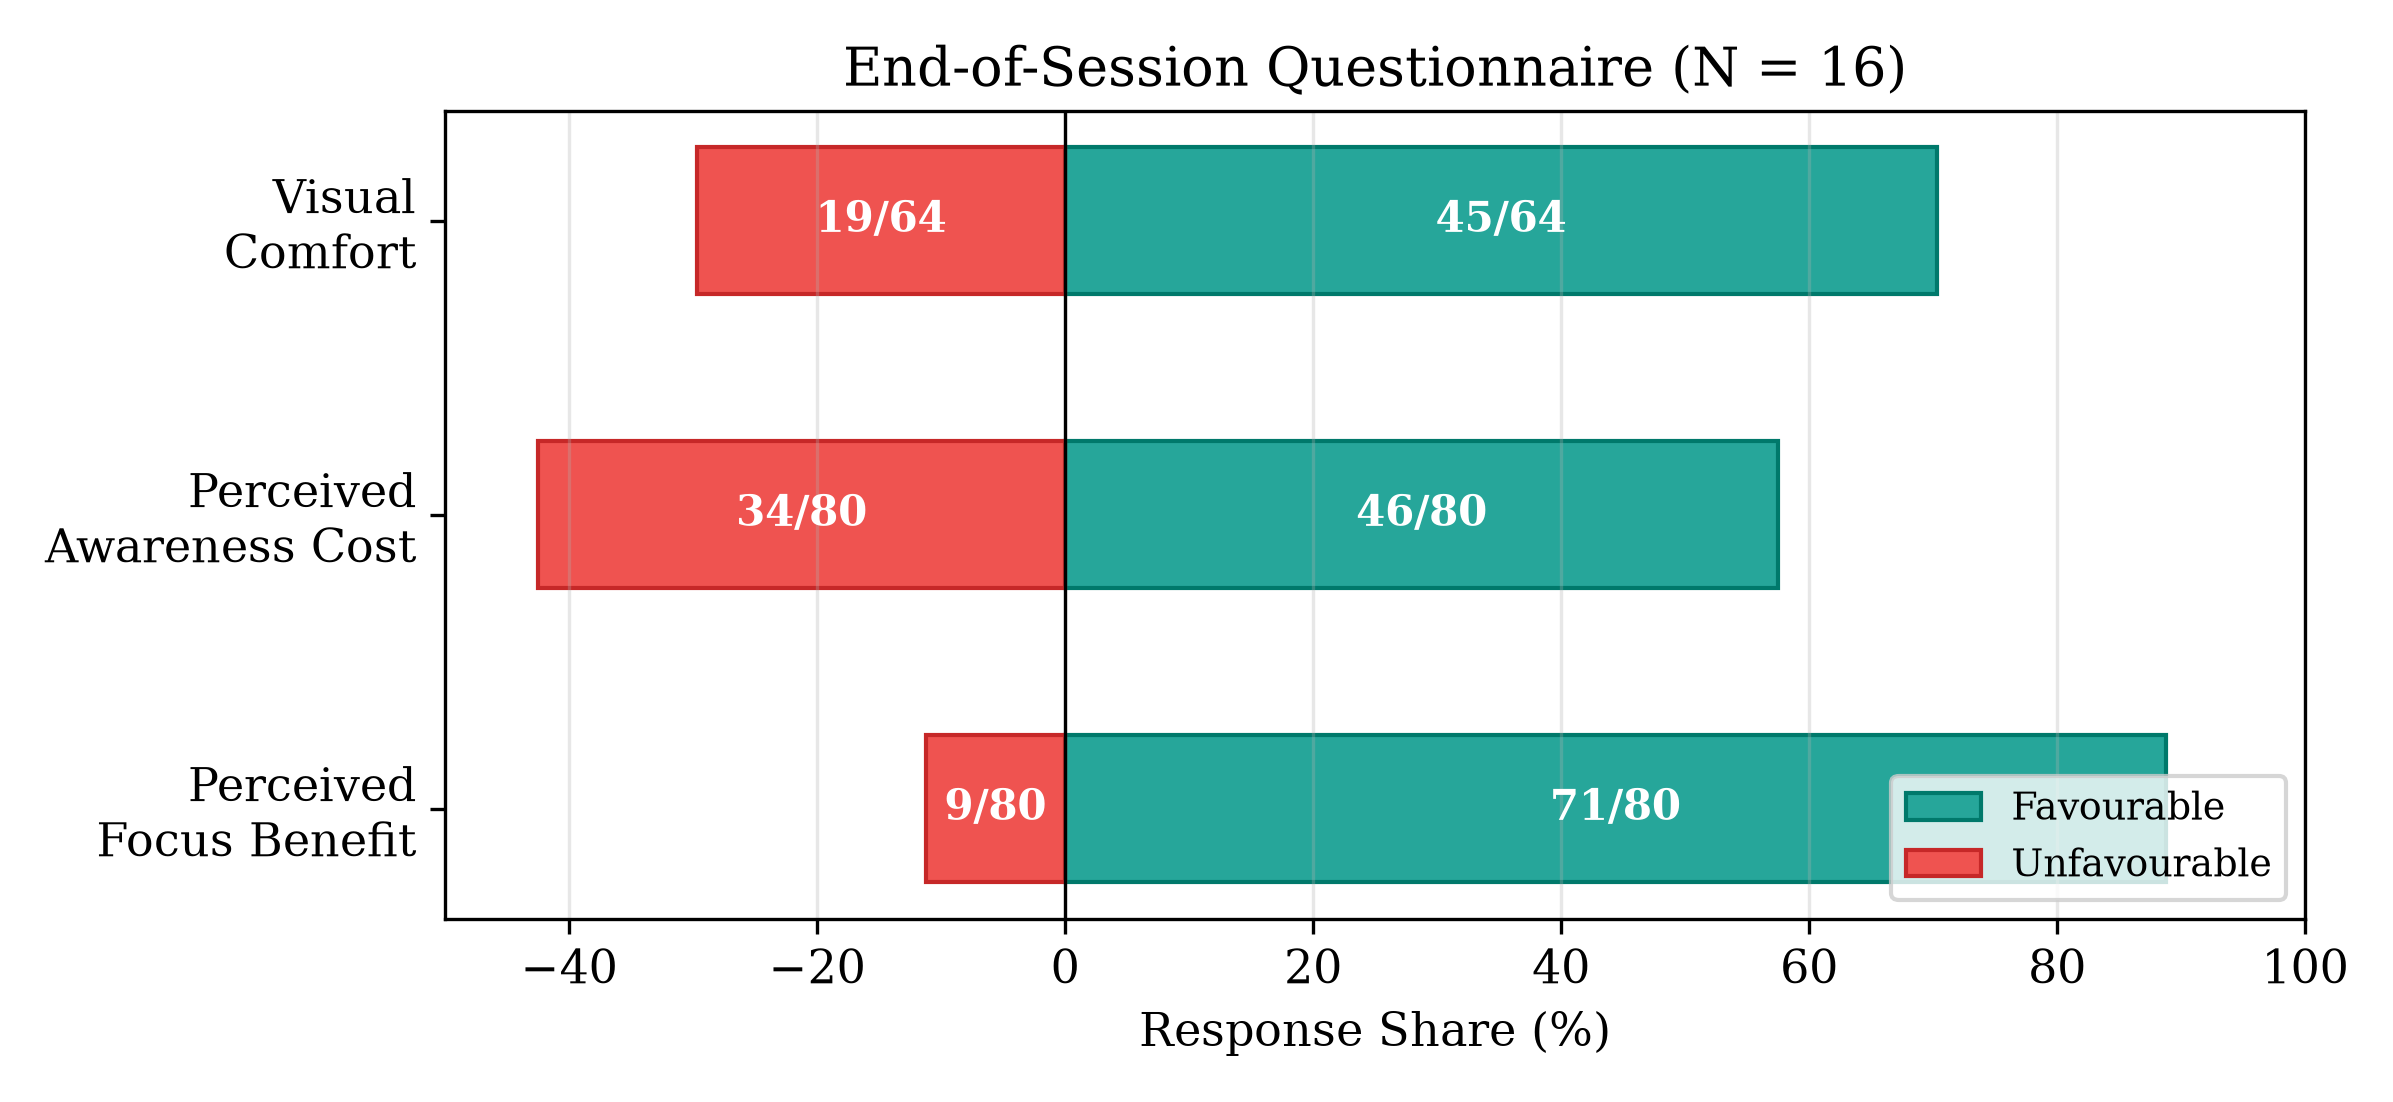
\includegraphics[width=\linewidth]{content/figures/fig_questionnaire.png}
\caption{End-of-session questionnaire responses by construct (N = 16).}
\label{fig:esq}
\end{figure}

\textbf{The subjective impression of lost awareness is not supported by the behavioural hit rate},
which shows no loss at all and, in the 20--30$^{\circ}$ band, an improvement. Two explanations are
worth taking seriously rather than explaining away. First, noticing that the periphery has been
changed is a different experience from missing something in it, and the DR manipulations studied to
date have all been reported as noticeable \citep{sutton2022}. ``I can tell my vision has been altered'' and ``I failed to detect
something'' are not the same report, even when only the first is true. Second, narrowed-field anxiety
is documented independently of task performance, rising in every restricted-field condition tested in
the literature, including conditions where spatial learning is unaffected \citep{barhorstcates2016}.
Reassuring people directly, for instance with a visible cue when something happens outside the
window, would reintroduce exactly the salience the filter exists to remove. That is the trade-off in
its sharpest form, and it is left unresolved here.

\subsection{What this result does and does not show}

Read against the decision table, the study lands on the working-system end of the range the
literature left open, with its verdicts stated at their honest strength. The primary contrast is a
real, adequately powered 3.09-point accuracy gain on a real-hardware task with real physical
distractors, surviving both a parametric and an assumption-free test, claimed as a bounded benefit
because its interval spans the pre-set half-the-errors bar (row 4). Peripheral awareness did not
drop: the worst case the data support is no loss to within a tenth of a point against a ten-point
margin, and raising pooled detection across the whole field was never SignPop's job, so the pooled
estimate's 50\% power bounds a secondary description, not a claim the design depends on. And
detection improved specifically where the mechanism predicted it would, in the pre-registered
20--30$^{\circ}$ band, at 84\% achieved power.

Three qualifications bound all of it. The sample is seventeen and fifteen pairs, not the
pre-registered twenty, so every interval is wider than the design intended and the shortfall stands
as a deviation however well the power figures absorbed it. The pooled Block B estimate carries the
response-criterion qualification of Section 5.7.2. And the bundle limitation of Chapter 4,
Section 4.5.5 applies in full, so nothing above attributes the 20--30$^{\circ}$ gain to any one of
the six effects a detection fires. Chapter 6 takes up what follows.
